% **** Szablon pracy magisterskiej, licencjackiej lub inżynierskiej ****

\documentclass[polish,12pt,twoside,a4paper]{report}
\renewcommand{\baselinestretch}{1.15} 

% *************** Definicje stylu dokumentu ***************

% *********************************************************************************
% W pliku tym zdefiniowany jest wygl¹d dokumentu.
% Zmiany tutaj nie s¹ konieczne o ile nie zamierzasz zmieniaæ wygl¹du dokumentu.
% *********************************************************************************

% *************** Za³adowanie pakietów ***************
\usepackage[a4paper,twoside,left=2.0cm,right=1.5cm,top=1.5cm,bottom=1.5cm]{geometry}
\usepackage[T1]{fontenc}
%\usepackage[cp1250]{inputenc}
\usepackage[utf8]{inputenc}
\usepackage[polish]{babel}
\usepackage{amsmath}
\usepackage{amsfonts}
\usepackage{graphicx}
\usepackage{graphics}
\usepackage{times}
\usepackage{indentfirst}%wciecia a nowych akapitach

\selectlanguage{polish}

%szerokoœœ wciêæ
\setlength{\parindent}{1.25cm}

%numeracja stron
\usepackage{fancyhdr}
\pagestyle{fancy}
\fancyhf{} % usun biezace ustawienia pagin
\fancyhead[LE,RO]{ }
\fancyhead[LO]{ }
\fancyhead[RE]{ }
\fancyfoot[CE,CO]{\small\thepage}
\fancyfoot[LO]{ }
\fancyfoot[RE]{ }
\renewcommand{\headrulewidth}{0.0pt}
\renewcommand{\footrulewidth}{0.0pt}
\addtolength{\headheight}{0.0pt} % pionowy odstep na kreske
\fancypagestyle{plain}{%
\fancyhead{} % usun p. górne na stronach pozbawionych
% numeracji (plain)
\renewcommand{\headrulewidth}{0.0pt} % pozioma kreska
\setlength{\headheight}{15pt}.
}

% *************** Definicje niektórych kolorów ***************
\usepackage{color}

\definecolor{greenyellow}   {cmyk}{0.15, 0   , 0.69, 0   }
\definecolor{yellow}        {cmyk}{0   , 0   , 1   , 0   }
\definecolor{goldenrod}     {cmyk}{0   , 0.10, 0.84, 0   }
\definecolor{dandelion}     {cmyk}{0   , 0.29, 0.84, 0   }
\definecolor{apricot}       {cmyk}{0   , 0.32, 0.52, 0   }
\definecolor{peach}         {cmyk}{0   , 0.50, 0.70, 0   }
\definecolor{melon}         {cmyk}{0   , 0.46, 0.50, 0   }
\definecolor{yelloworange}  {cmyk}{0   , 0.42, 1   , 0   }
\definecolor{orange}        {cmyk}{0   , 0.61, 0.87, 0   }
\definecolor{burntorange}   {cmyk}{0   , 0.51, 1   , 0   }
\definecolor{bittersweet}   {cmyk}{0   , 0.75, 1   , 0.24}
\definecolor{redorange}     {cmyk}{0   , 0.77, 0.87, 0   }
\definecolor{mahogany}      {cmyk}{0   , 0.85, 0.87, 0.35}
\definecolor{maroon}        {cmyk}{0   , 0.87, 0.68, 0.32}
\definecolor{brickred}      {cmyk}{0   , 0.89, 0.94, 0.28}
\definecolor{red}           {cmyk}{0   , 1   , 1   , 0   }
\definecolor{orangered}     {cmyk}{0   , 1   , 0.50, 0   }
\definecolor{rubinered}     {cmyk}{0   , 1   , 0.13, 0   }
\definecolor{wildstrawberry}{cmyk}{0   , 0.96, 0.39, 0   }
\definecolor{salmon}        {cmyk}{0   , 0.53, 0.38, 0   }
\definecolor{carnationpink} {cmyk}{0   , 0.63, 0   , 0   }
\definecolor{magenta}       {cmyk}{0   , 1   , 0   , 0   }
\definecolor{violetred}     {cmyk}{0   , 0.81, 0   , 0   }
\definecolor{rhodamine}     {cmyk}{0   , 0.82, 0   , 0   }
\definecolor{mulberry}      {cmyk}{0.34, 0.90, 0   , 0.02}
\definecolor{redviolet}     {cmyk}{0.07, 0.90, 0   , 0.34}
\definecolor{fuchsia}       {cmyk}{0.47, 0.91, 0   , 0.08}
\definecolor{lavender}      {cmyk}{0   , 0.48, 0   , 0   }
\definecolor{thistle}       {cmyk}{0.12, 0.59, 0   , 0   }
\definecolor{orchid}        {cmyk}{0.32, 0.64, 0   , 0   }
\definecolor{darkorchid}    {cmyk}{0.40, 0.80, 0.20, 0   }
\definecolor{purple}        {cmyk}{0.45, 0.86, 0   , 0   }
\definecolor{plum}          {cmyk}{0.50, 1   , 0   , 0   }
\definecolor{violet}        {cmyk}{0.79, 0.88, 0   , 0   }
\definecolor{royalpurple}   {cmyk}{0.75, 0.90, 0   , 0   }
\definecolor{blueviolet}    {cmyk}{0.86, 0.91, 0   , 0.04}
\definecolor{periwinkle}    {cmyk}{0.57, 0.55, 0   , 0   }
\definecolor{cadetblue}     {cmyk}{0.62, 0.57, 0.23, 0   }
\definecolor{cornflowerblue}{cmyk}{0.65, 0.13, 0   , 0   }
\definecolor{midnightblue}  {cmyk}{0.98, 0.13, 0   , 0.43}
\definecolor{navyblue}      {cmyk}{0.94, 0.54, 0   , 0   }
\definecolor{royalblue}     {cmyk}{1   , 0.50, 0   , 0   }
\definecolor{blue}          {cmyk}{1   , 1   , 0   , 0   }
\definecolor{cerulean}      {cmyk}{0.94, 0.11, 0   , 0   }
\definecolor{cyan}          {cmyk}{1   , 0   , 0   , 0   }
\definecolor{processblue}   {cmyk}{0.96, 0   , 0   , 0   }
\definecolor{skyblue}       {cmyk}{0.62, 0   , 0.12, 0   }
\definecolor{turquoise}     {cmyk}{0.85, 0   , 0.20, 0   }
\definecolor{tealblue}      {cmyk}{0.86, 0   , 0.34, 0.02}
\definecolor{aquamarine}    {cmyk}{0.82, 0   , 0.30, 0   }
\definecolor{bluegreen}     {cmyk}{0.85, 0   , 0.33, 0   }
\definecolor{emerald}       {cmyk}{1   , 0   , 0.50, 0   }
\definecolor{junglegreen}   {cmyk}{0.99, 0   , 0.52, 0   }
\definecolor{seagreen}      {cmyk}{0.69, 0   , 0.50, 0   }
\definecolor{green}         {cmyk}{1   , 0   , 1   , 0   }
\definecolor{forestgreen}   {cmyk}{0.91, 0   , 0.88, 0.12}
\definecolor{pinegreen}     {cmyk}{0.92, 0   , 0.59, 0.25}
\definecolor{limegreen}     {cmyk}{0.50, 0   , 1   , 0   }
\definecolor{yellowgreen}   {cmyk}{0.44, 0   , 0.74, 0   }
\definecolor{springgreen}   {cmyk}{0.26, 0   , 0.76, 0   }
\definecolor{olivegreen}    {cmyk}{0.64, 0   , 0.95, 0.40}
\definecolor{rawsienna}     {cmyk}{0   , 0.72, 1   , 0.45}
\definecolor{sepia}         {cmyk}{0   , 0.83, 1   , 0.70}
\definecolor{brown}         {cmyk}{0   , 0.81, 1   , 0.60}
\definecolor{tan}           {cmyk}{0.14, 0.42, 0.56, 0   }
\definecolor{gray}          {cmyk}{0   , 0   , 0   , 0.50}
\definecolor{black}         {cmyk}{0   , 0   , 0   , 1   }
\definecolor{white}         {cmyk}{0   , 0   , 0   , 0   } 

% *************** Koniec definicji stylu dokumentu ***************


%definicja przydatnych poleceń
\newcommand{\wydzial}{KOLEGIUM INFORMATYKI STOSOWANEJ}
\newcommand{\kierunek}{Kierunek: INFORMATYKA}
\newcommand{\specjalnosc}{Specjalność: Teleinformatyka}
\newcommand{\autor}{Imię nazwisko}
\newcommand{\album}{Nr albumu studenta 213767}
\newcommand{\nauczyciel}{imię nazwisko}
\newcommand{\tematprojektu}{TEMAT PROJEKTU}
\newcommand{\miasto}{Rzeszów}
\newcommand{\przedmiot}{Przedmiot}
\newcommand{\rok}{2026}

\begin{document}

% *************** Włączenie definicji pierwszych stron ***************
% *************** Strony tytułowe ***************

% ************************************************************
% W tym miejscu znajduje sie definicja wyglądu pierwszych stron:
% strony tytułowej, strony z oświadczeniem o treści pracy
% i strony ze spisem treści
% ************************************************************
% *************** Strona tytułowa ***************
%umieszczenie logo i nazwy uczelni
\noindent
\parbox{65mm}{
\includegraphics[width=13.0cm, height=3.0cm]{logoWSIiZ}}

\vspace{10mm}
\begin{center}
{\Large{}\textbf{\wydzial}}
\end{center}
\vspace{10mm}
\noindent
\hspace{30mm}{\Large{}\textbf{\kierunek}}\\

\noindent
\hspace{30mm}{\Large{}\textbf{\specjalnosc}}
\vspace{30mm}
\begin{center}
	{\large{}\autor}\\
	{\large{}\album}\\
	\vspace{15pt}
	{\huge{}\textbf{Projekt z przedmiotu ,,\przedmiot''}}\\
	\vspace{20pt}
	{\normalsize{}Prowadzący: \nauczyciel}\\
	\vspace{100pt}
	{\LARGE{}\textbf{\tematprojektu}}\\
	\vspace{190pt}
	{\large{}\textbf{\miasto {} \rok}}
\end{center}

% pusta zawartość stopki - brak numeru strony
\thispagestyle{empty}

% *************** Strona z oświadczeniem o treści pracy ***************
\newpage
\text{}

\thispagestyle{empty}
\newpage


% *************** Spis treści ***************
\tableofcontents
% pusta zawartość stopki - brak numeru strony
\thispagestyle{empty}
\newpage

% *************** Koniec pliku front.tex ***************



% *************** Część główna pracy ***************
\chapter*{Wstęp}

Sieci oparte o stos TCP/IP są dominującym rozwiązaniem w Internecie i wykorzystywane w sieciach lokalnych i rozległych. Niestety pula adresów IPv4 wyczerpała się \cite{www-1} powodując konieczność wdrażania IPv6. Rysunek \ref{fig:plotend} przedstawia przewidywania dalszego wykorzystania adresacji IPv4.

\begin{figure}[!ht]
	\centering
		
	\caption{\footnotesize Przewidywania dotyczące alokacji adresów IPv4. Żródło: \cite{www-1}}
        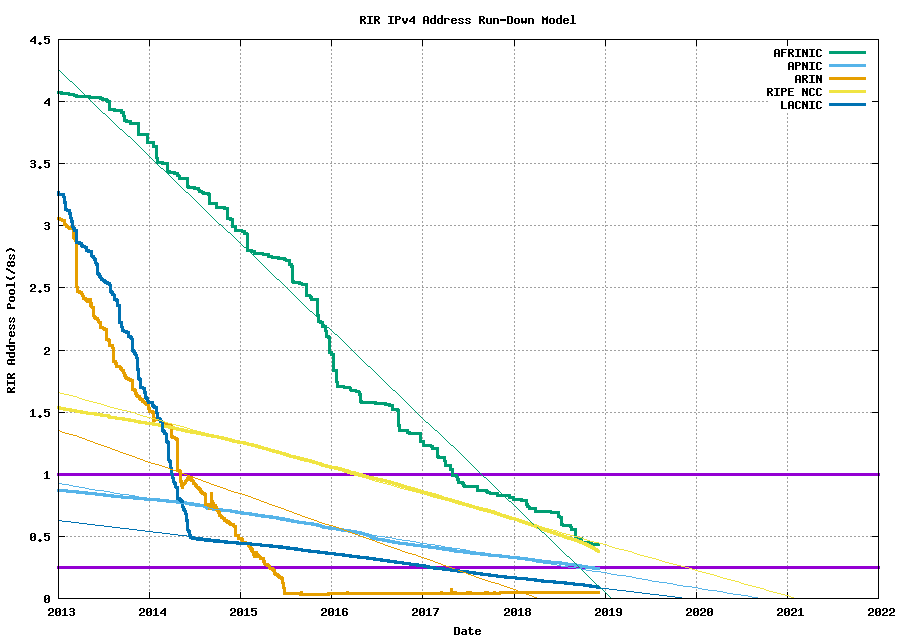
\includegraphics[width=16cm]{figures/plotend.png}
	\label{fig:plotend}
\end{figure}

Sukcesywne wdrażanie IPv6 stało się faktem. Są kraje w których ponad połowa użytkowników Internetu używa IPv6 \cite{www-2}. Tabela \ref{tab:KrajeZ} przedstawia dane krajów w których wdrożenie jest najbardziej zaawansowane oraz polski.

\begin{table}[!ht]
	\caption{\footnotesize Kraje z najbardziej zaawansowanym stanem wdrozenia IPv6.}
		\begin{center}
			\begin{small}
				\begin{tabular}{|l|l|l|l|l|l|l|}
					\hline
					Index&ISO-3166 &Internet Users&V6 Use &V6 Users &Population&Country \\
							 & Code &                 & ratio & (Est) &   & \\
					\hline
					1&BE&10228360&58.14&5946437&11557470&Belgium \\
					2&IN&475642226&52.49&249647006&1366788008&India \\
					3&US&290930388&42.11&122497974&328734902&United States of America \\ 
					4&DE&72552125&41.35&30002918&82445597&Germany \\
					\hline
				
				\end{tabular}
			\end{small}
			\end{center}
	\label{tab:KrajeZ}
\end{table}
\addcontentsline{toc}{chapter}{Wstęp}
\newpage
% ********** Rozdział 1 **********
\chapter{Tytuł pierwszego rozdziału}
\section{Tytuł pierwszego punktu}
\subsection{Tytuł pierwszego podpunktu}

Tutaj powinien zostać umieszczony tekst. Poniższe akapity stanowią zastosowanie możliwości składania tekstu, tabel, grafiki i wyrażeń matematycznych w systemie \LaTeX.

\subsection{Przypisy}\label{przypisy}. 
Pierwszym spisanym polskim zdaniem jest: ,,Day, ut ia pobrusa, a ti poziwai''\footnote{Zdanie pochodzi z Księgi henrykowskiej. Zostało spisane w 1270 roku. Wypowiedział je osiadły na Dolnym Śląsku czeski rycerz Boguchwał do jego miejscowej żony, gdy ta mełła ziarno na ręcznych żarnach. Znajduje się ono w opisie pochodzenia należącej do dóbr klasztornych pobliskiej wsi Brukalice. Jako że mielenie ziarna było wtedy uważane za pracę niegodną mężczyzny, Czech ten został nazwany przez sąsiadów Brukałą (zbrukany), a przezwisko to dało także miano całej osadzie.}, co znaczy: ,,Daj, ja będę mełł, a ty odpocznij'' (Daj, niech ja pokręcę żarna, a ty odpocznij).

\subsection{Wyróżnienia i kroje pisma}
\noindent
Tekst nieformatowany.\\
\textbf{Tekst pogrubiony.}\\
\textit{Tekst pochylony.}\\
\underline{Tekst podkreślony.}\\
\textbf{\textit{Tekst pogrubiony i pochylony, }\underline{a teraz pogrubiony i podkreślony}}\\ \\
{\bf Tekst pogrubiony. }
{\it Tekst pochylony. }
\emph{Wyróżnienie}\\
\textsc{Kapitaliki}\\
\texttt{Grotesk}\\
\textsf{Krój bezszeryfowy}\\
\textrm{Krój szeryfowy }\\

\subsection{Stopnie czcionek}
\noindent {\tiny tiny} {\scriptsize scriptsize} {\footnotesize footnotesize} {\small small} {\normalsize normalsize} {\large large} {\Large Large} {\LARGE LARGE} {\huge huge} {\Huge Huge}

\subsection{Kolory}
\textcolor{red}{Czerwony} \textcolor{green}{zielony} \textcolor{blue}{niebieski.} A teraz \colorbox{yellow}{tekst na żółtym tle}.

\subsection{Pozycjonowanie tekstu}
\begin{flushleft}
Tekst wyrównany do lewego marginesu.\\
\end{flushleft}
\begin{flushright}
Tekst wyrównany do prawego marginesu.\\
\end{flushright}
\begin{center}
Tekst wyrównany do środka strony.\\
\end{center}

\subsection{Wyliczenia i wypunktowania}
\begin{enumerate}
\item pozycja enumerate 1
	\begin{enumerate}
	\item pozycja enumerate a
		\begin{enumerate}
			\item pozycja enumerate i
		\end{enumerate}
	\end{enumerate}
\begin{itemize}
	\item[a)] wyliczenie 1
	\item[--] wyliczenie 3
	\item[*] wyliczenie 4
\end{itemize}

\item pozycja enumerate 2
\begin{description}
		\item[pozycja] description 1
\end{description}
\end{enumerate}

\subsection{Inne otoczenia}
Poniżej widać przykład zastosowania otoczenia verbatim.
\begin{verbatim}
\begin{enumerate}
\item pozycja enumerate 1
	\begin{enumerate}
	\item pozycja enumerate a
		\begin{enumerate}
			\item pozycja enumerate i
		\end{enumerate}
	\end{enumerate}
\end{verbatim}

{\verb*#Zastosowanie polecenia {\verb*?tekst?}#}. 

\subsection{Etykiety i odsyłacze}\label{etykiety}
Jest to przykład zastosowania etykiet i odsyłaczy. Obecnie znajdujemy się w podpunkcie \ref{etykiety}. Podpunkt "Przypisy" ma numer \ref{przypisy}. Rysunek \ref{fig:plotend} pochodzi z \cite{www-1}.


\subsection{Tabele}
Wzór tabeli jaki należy stosować w pracy dyplomowej. Naturalnie rodzaj wyrównania tekstu w tabeli zależy od użytkownika.
\begin{table}[!ht]
	\begin{center}
	\caption{{\footnotesize Opis tabeli}}
	%Definicja tabeli w otoczeniu tabular
	\begin{small}
	\begin{tabular}{|l|c|r|} \hline
	Kolumna 1 & Kolumna 2 & Kolumna 3 \\ \hline
	1 & 2 & 3 \\ \hline
	2 & 3 & 4 \\ \hline
	3 & 4 & 5 \\ \hline
	\end{tabular}
	\end{small}
	\end{center}
\end{table}

\subsection{Rysunki}
Wzór rysunku jaki należy stosować w pracy dyplomowej.
Rysunek został umieszczony na górze strony celem lepszego dopasowania składanego tekstu.
\begin{figure}[!ht]
	\begin{center}
        \caption{{\footnotesize Opis rysunku}}
	
\includegraphics[width=4cm, height=3cm, angle=45]{logoWSIiZ}
	\end{center}
\end{figure}

\subsection{Wyrażenia matematyczne}
Najsłynniejszy wzór Alberta Einsteina opublikowany w 1905 roku: \(E=mC^{2}\). 
Wzór opisuje równoważność masy i energii.
\[ E=mC^{2} \]
\begin{displaymath}E=mC^{2}\end{displaymath}
To samo tylko z numeracją wzorów
\begin{equation}E=mC^{2}\end{equation}

\begin{equation}P\left(\bigcup_{i=1}^{\infty}{A_i} \right)=\sum_{i=1}^{\infty}{P(A_i)}\end{equation}

\subsection{Czcionki w wyrażeniach matematycznych}
\noindent
\[ \mathrm{aAbBcCdDeEfFgGhHiIjJkKlLmMnNoOpPqQrRsStTuUvVwWxXyYzZ} \]
\[ \mathnormal{aAbBcCdDeEfFgGhHiIjJkKlLmMnNoOpPqQrRsStTuUvVwWxXyYzZ} \]
\[ \mathcal{ABCDEFGHIJKLMNOPQRSTUVWXYZ} \]
\[ \mathfrak{aAbBcCdDeEfFgGhHiIjJkKlLmMnNoOpPqQrRsStTuUvVwWxXyYzZ} \]
\[ \mathbb{ABCDEFGHIJKLMNOPQRSTUVWXYZ} \]

% ********** Koniec rozdziału **********

\newpage
% ********** Rozdział 2 **********
\chapter{Tytuł rozdziału}


\section{Tytuł punktu}
\subsection{Tytuł podpunktu}
\subsubsection{Tytuł podpodpunktu}
Tekst

% ********** Koniec rozdziału **********

\newpage
% ********** Rozdział 3 **********
\chapter{Tytuł trzeciego rozdziału}
\section{Tytuł punktu}
\subsection{Tytuł podpunktu}
\subsubsection{Tytuł podpodpunktu}
Tekst

% ********** Koniec rozdziału **********

%*** W razie potrzeby dodaj pozostałe rozdziały ***%
\end{document}
% *************** Koniec pliku szablon.tex ***************
